\documentclass[journal]{IEEEtran}
\usepackage{graphicx}
\usepackage{array}

\ifCLASSINFOpdf
  % \usepackage[pdftex]{graphicx}
  % \DeclareGraphicsExtensions{.pdf,.jpeg,.png}
\else
  % \DeclareGraphicsExtensions{.eps}
\fi

%\hyphenation{op-tical net-works semi-conduc-tor}

\begin{document}
\title{Delivering Reliable Software in the European Scientific Arena: Evolution of Methodologies and New Trend Analysis}
%\title{15 years of European scientific software development: evolution and methodologies}

\author{E. Ronchieri,
        P. Orviz Fernandez,
        M. David,
		D. C. Duma,
        J. Gomes,
        D. Salomoni
\thanks{D. C. Duma, E. Ronchieri, and D. Salomoni are with INFN - CNAF, Bologna, Italy.}
\thanks{P. Orviz Fernandez, is with CSIC, Santander, Spain, (e-mail: orviz@ifca.unican.es)}
\thanks{M. David, and J. Gomes are with LIP, Lisbon, Portugal.}%
}

% The paper headers
%\markboth{IEEEtran for IEEE Journals}

\maketitle

\begin{abstract}
From the advent of Grid technology as the new paradigm of distributed
computing to the current days of Cloud computing models, the continuous need
of new tools and services to match the scientific community requirements has been
addressed in Europe by the creation of software development and
e-Infrastructure coordination dedicated projects. This work examines the
evolution of the software engineering methodologies used in past and present
European Commission-funded software projects to illustrate how the research on software
reliability has progressed in Europe over the last 15 years following the
foundation of the first project in 2001. In particular, we describe the team
organizational structure, techniques and procedures that have guided the Quality
Assurance definitions in order to deliver quality software. We highlight the challenges
and barriers that have been faced throughout these years and how to overcome them totally or
partially. To conclude, we discuss the future directions of software
Quality Assurance methodologies for the incoming projects.
\end{abstract}

\begin{IEEEkeywords}
Software Reliability, Quality Assurance, Software Metrics, Software Testing
Techniques
\end{IEEEkeywords}

\IEEEpeerreviewmaketitle

\section{Introduction}

\IEEEPARstart{A}{n}alyzing the European Commission-funded software projects in the last decade we have observed a continuous
increase of the prominence and robustness of testing and validation procedures. The first of many reasons is related to the evolution of the software engineering
techniques (e.g. rise of DevOps practices \cite{zhu}) together with the parallel advancements in the ICT field with virtualization and container
technologies. Another one is the emergence of automation and event-response tools. 

Software developers involved in these projects over time have learned  how to make their final products more reliable in order to satisfy requirements of different communities, such as physics.

In this paper, we introduce a set of European Commission (EC)-funded projects that goes from
2001 up to now, where the authors of this summary were and are currently
involved. For each project, we explain how they addressed the challenge in
software reliability. Furthermore, we detail new trends in software reliability.

The reminder of this paper is organized as follows. Section \ref{sec:ev} details the evolution of research on software reliability in EC-projects. Section \ref{sec:ntsr} provides information about new research trends in software reliability. Finally, Section \ref{sec:con} concludes. 

\section{Evolution of research on software reliability in EC-projects}
\label{sec:ev}

In the following we provide an overview of the main EC-projects that have dealt with the issue of software reliability. Table \ref{tab:eup} shows the various projects with their logo, short name, long name and duration.

\begin{table}[!h]
%% increase table row spacing, adjust to taste
\renewcommand{\arraystretch}{1.3}
% if using array.sty, it might be a good idea to tweak the value of
% \extrarowheight as needed to properly center the text within the cells
\caption{List of EC-projects}
\label{tab:eup}
\centering
%% Some packages, such as MDW tools, offer better commands for making tables
%% than the plain LaTeX2e tabular which is used here.
\begin{tabular}{p{1.6cm}p{1.5cm}p{3cm}l}
\hline
\hline
\\
Logo & Short Name & Long Name & Duration\\
\hline
\hline
\begin{minipage}{.3\textwidth}

\includegraphics[width=15mm,height=7.5mm]{images/datagrid}
\end{minipage}
    & DataGrid &
Research and Technological Development for an International Data GridTwo & 2001--2004\\
\begin{minipage}{.3\textwidth}

\includegraphics[width=15mm,height=7.5mm]{images/egee}
\end{minipage}
     & EGEE I, II, III &
Enabling Grids for E-sciencE & 2004--2010\\
\begin{minipage}{.3\textwidth}

\includegraphics[width=15mm,height=7.5mm]{images/etics}
\end{minipage}
     & ETICS 1, 2 &
E--Infrastructure for Testing, Integration and Configuration of Software & 2006-2010\\
\begin{minipage}{.3\textwidth}

\includegraphics[width=15mm,height=7.5mm]{images/emi}
\end{minipage}
     & EMI &
Europeean Middleware Initiative & 2010--2013\\
\begin{minipage}{.3\textwidth}

\includegraphics[width=15mm,height=7.5mm]{images/egi}
\end{minipage}
     & EGI-Inspire &
Integrated Sustainable Pan-European Infrastructure for Researchers in Europe
 & 2010--2014\\
\begin{minipage}{.3\textwidth}

\includegraphics[width=15mm,height=7.5mm]{images/indigo}
\end{minipage}
     & INDIGO-DataCloud &
INtegrating Distributed data Infrastructures for Global ExplOitation
 & 2015--2017\\
\hline
\hline
\end{tabular}
\end{table}



\subsection{DataGrid}

The DataGrid \cite{cordis:datagrid} project (Jan 2001 -- Dec 2003) was devoted
to develop the first European infrastructure for Grid computing. The project
brought together 21 academic and industry partners, from 15 different
countries. There were 3 application areas for requirement gathering;
Particle physics, Bioinformatics and Earth observation. The project delivered
their own software distribution, named EDG (EU DataGrid), strongly based on
Globus Middleware Services \cite{globus}. The development organization
consisted in 5 work packages coordinated by an Architecture Task Force,
supervising the overall design and technical consistency of the developments.

Due to having no previous experience in such widely
collaborative projects, a big effort was spent trying to devise solutions for several
challenges \cite{datagrid}, namely the 1) communication overhead, as a
result of the large geographical separation of the parties involved in the
development tasks, 2) the evolution of the requirements coming from the user
communities, and 3) the lack of a body of knowledge for academic software
engineering.

Agile methodologies were being introduced at the time
through the Agile manifesto \cite{agile-manifesto}, as such the project's
development design suffered from the methods, tools, techniques and best
practices emerging from the new discipline of software engineering
\cite{agile}. Nonetheless, the project focused on the experiences and procedures
from open source software projects, such as Linux and Apache, trying to reach a
higher maturity level \cite{cmm}.

\subsection{Enabling Grids for E--sciencE}

The three phases of Enabling Grids for E--sciencE (EGEE, Apr 2004 -- Apr 2010)
\cite{cordis:egee, cordis:egee2, cordis:egee3} projects brought together
scientists and engineers from more than 240 institutions in 45 countries to
provide a seamless Grid infrastructure for e--Science. EGEE--II and EGEE--III
featured the internationalization of the project, embracing worldwide research
institutions and user communities. The software to sustain the increasing
requirements from the diverse scientific communities would need to develop a
rich set of new services while maintaining a sustainable infrastructure for
Grid computing, eventually used by more than 15 thousand researchers and deployed in
over 250 institutions.

The {\sl gLite} middleware \cite{glite} was the ultimate
official distribution of EGEE as of 2006, after two years of prototyping and
re--engineering efforts to converge with LHC Computing Grid (LCG--2), Virtual
Data Toolkit (VDT) and Condor \cite{condor} software distributions. The
development team was comprised of more that 80 people from 12 academic and
industrial partners, that issued more than 10 thousand bugs, 1.7 thousand patches and
defined over 300 tasks tracked by the use of bug/task management tools.

The
source code was available at a private, centralized version control system.
The code was not validated by any Quality Assurance policy, but passed through a manual
certification procedure at the time of the release. This procedure tried to
improve the reliability of the software components by applying a set of
requirements [ref] to be fulfilled at each stage (integration, certification,
pre--production, production), carried out by different teams. However, starting in
EGEE--II, the project adopted the ETICS solution, aiming to develop
an automatic build system for Grid middleware.

\subsection{E--Infrastructure for Testing, Integration and Configuration of Software}

The E--Infrastructure for Testing, Integration and Configuration of Software
\cite{cordis:etics, cordis:etics2} (ETICS, Jan 2006 -- Feb 2010) project aimed
at addressing the challenges in producing quality software in distributed,
collaborative projects such as EGEE and its gLite middleware. The framework
integrated different technologies and tools to provide automated configuration,
build and testing capabilities, as well as auto-generated documentation and
software metrics gathering such as Source Lines Of Code (SLOC), complexity and
number of defects/bugs \cite{etics}. The ETICS portal was the first automated
service for delivering software products in distributed environments like
the Grids.

\subsection{European Middleware Initiative}

The European Middleware Initiative (EMI, May 2010 -- Apr 2013)
\cite{cordis:emi} project joined the 4 major Grid middleware providers in
Europe at the time -- {\sl gLite}, {\sl UNICORE}, {\sl ARC} and {\sl dCache} --
to maintain and evolve the middleware focusing on extending the
interoperability in the Grid and improving the reliability of the services. The
ISO/IEC 9126 \cite{iso-9126} standard was used in order to identify a set of
characteristics that needed to be present in the EMI software products and
processes to be able to meet the EMI quality requirements
\cite{emi-quality-model}.

For each software characteristic, a set of associated
metrics and Key Performance Indicators (KPIs) were identified and defined in
detail in the EMI Metrics Specification \cite{emi-metrics}. The project
leveraged the {\sl ETICS} service for the development and release management,
as well as for metric tracking, making queries on the collected data to display
them through the chart generation framework.

\subsection{EGI--Integrated Sustainable Pan--European Infrastructure}


The EGI--InSPIRE (Integrated Sustainable Pan--European Infrastructure for
Researchers in Europe, May 2010 -- May 2014) project \cite{cordis:egi-inspire}
arose as the continuation of the EGEE--III project, establishing and
maintaining a sustainable European Grid Infrastructure.

EGI--InSPIRE did not
develop any software but maintained a production--ready Grid computing
middleware distribution called {\sl UMD} (Unified Middleware Distribution).
The role of {\sl UMD} was to enforce the fulfilment of a set of quality
criteria definitions \cite{egi-qc} in the software being delivered (i.e.,
{\sl EMI} and {\sl Globus}) \cite{mario}. {\sl UMD} is still being used and
deployed in the European scientific e--Infrastructures under a follow--up
project, the EGI--Engage (Engaging the EGI Community towards an Open Science
Commons) \cite{cordis:egi-engage}. This distribution is currently complemented
by a Cloud--specific one called {\sl CMD} (Cloud Middleware Distribution).

\subsection{INtegrating Distributed data Infrastructures for Global
ExplOitation}

The INDIGO-DataCloud (INtegrating Distributed data Infrastructures for Global
ExplOitation, Apr 2015 -- Sep 2017) \cite{cordis:indigo} is the last
project of software development considered in this review. At the time of writing
the project is succeeding in providing solutions to address the existing gaps in
cloud Platform--as--a--Service (PaaS) and Software--as--a--Service (SaaS) levels,
helping developers, e--Infrastructures and scientific communities to exploit
Cloud computing benefits.

\section{New trends in software reliability}
\label{sec:ntsr}

The INDIGO--Datacloud project reflects the progress made in software
quality and reliability aspects throughout the past scientific European
experiences. Nevertheless, the project’s Quality Assurance procedures are also
highly influenced by the insights of current big worldwide collaborations of
software development. These collaborations have continuously inspired new
technologies and procedures to increase the robustness and quality of the
software being delivered. In this scenario, the DevOps culture is one of the
major outcomes that has been progressively adopted in the INDIGO--DataCloud
project.

\subsection{DevOps practices}
\label{sec:devops}

The DevOps methods emphasize on exercising Quality Assurance techniques to
avoid infrastructure disruption whenever new developments are deployed into
production. The INDIGO--DataCloud project promoted the application of a Continuous Integration (CI)
scenario to enforce the Quality Assurance requirements for any piece of
software being produced within the project. Such environment requires an
automated ready--to--go infrastructure where the different services involved
(source code management platform, automation server) interact with each other
to trigger the quality check execution and return back the exit codes, together
with their outputs. To accomplish this, the project leveraged on tightly
integrated open source tools such as GitHub and Jenkins, as well as relying on
Docker container provisioning to speed up the source code validation. This CI
approach is guiding the project’s software development phase throughout the
first and second major releases.

As DevOps suggests, frequent releases positively affects the reliability of the
software. The software updates of INDIGO--DataCloud products taking place since
the second major release are passing through a Continuous Delivery (CD)
pipeline that adds the packaging of the software right after the execution of
the quality checks (as part of the CI).

The steps defined within the CD
pipeline differ whether the software is to be distributed in the form of Docker
images or via operating system’s packages. In the latter case an extra
validation step is added, consisting in the product’s deployment using a
Configuration Management (CM) solution. The installation uses the packages
built in the previous step and uploaded to a testing
repository. In the case of Docker images, the CM is used to build the image
itself, installing and configuring the product before uploading it to the
DockerHub repository \cite{indigo-dockerhub}. Figure \ref{fig:fig_CD} shows
the workflow followed by the products distributed as Docker images.

\begin{figure*}
\centering
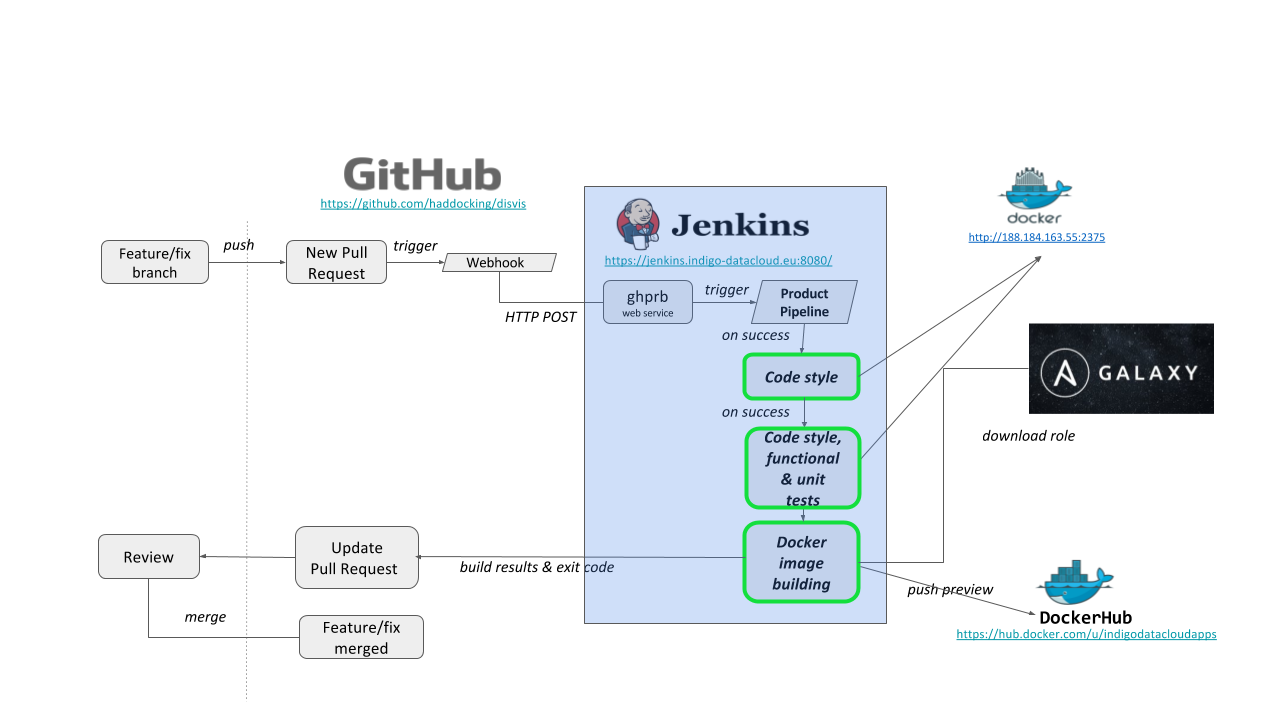
\includegraphics[width=\textwidth]{images/devops.png}
\caption{Continuous Delivery workflow for Docker images.}
\label{fig:fig_CD}
\end{figure*}

\subsection{Software Quality Procedures}

The software quality procedures \cite{indigo-d31} cover: 1) the identification
and description of the \emph{quality requirements} that the software need to
comply with, and 2) the \emph{quality metrics}.

The requirements are applied at early stages in the software development
process, integrated in the Jenkins CI service \cite{indigo-jenkins}, so that any
bug or design issue is likely to be detected and corrected promptly. The source
code is publicly available in GitHub repositories under an organization called
{\sl indigo-dc} \cite{indigo-github} to increase the visibility of the product
catalogue, promoting the external contributions and software adoption. Furthermore,
the source code is compliant with community de--facto style standards,
selected from the variety of programming languages being used as seen in
Fig. \ref{fig:fig_codestyle}.

\begin{figure}[!t]
\centering
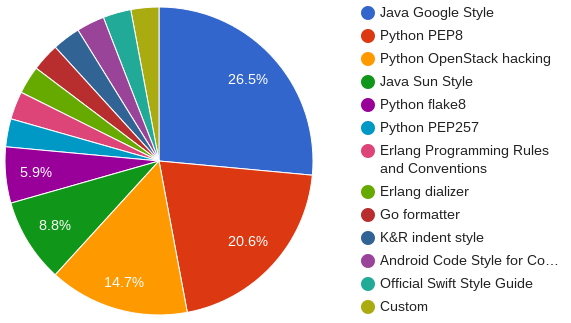
\includegraphics[width=0.5\textwidth]{images/codestyle.png}
\caption{Code style standards followed by INDIGO--DataCloud's software products.}
\label{fig:fig_codestyle}
\end{figure}

Unit testing coverage has increased between the first ({\sl INDIGO-1}) and the
second ({\sl INDIGO-2}) INDIGO--DataCloud releases, reaching an average value of
66.69\% on the {\sl INDIGO-2} release, very close to the recommended 70\% threshold
defined by the project’s SQA base criteria \cite{indigo-d31}. A comparison graph
between the code coverage for the products involved both in {\sl INDIGO-1} and
{\sl INDIGO-2} releases is shown in Fig. \ref{fig:fig_unittest}. As it can be seen,
a very small set of products with low coverage values highly impacted the overall
result, although a significant part of these products are upstream contributions
or products with codebases not fully under the control of the project. Nevertheless,
60\% of the products were over this threshold while 80\% of them have values above
the 50\% coverage.

The documentation of the products is treated as source code, using a markup
language, automatically rendered and uploaded to online repositories
\cite{indigo-gitbook}. Changes in both documentation and source code are
human--reviewed as the last step before merging them into the production
repository.

Last but not least, as described in section \ref{sec:devops}, in order
to facilitate the usage of the INDIGO--DataCloud services, they can be deployed
automatically using either Ansible \cite{indigo-ansible} or Puppet
\cite{indigo-puppet} open--source tools. The adoption of such Configuration Management
tools not only eases the consumption of the products developed by external users or
infrastructures, but also tackles the correct installation and configuration of the
services and applications. A representative example is the number of roles currently
hosted in the Ansible Galaxy portal for the project.

\begin{figure*}
\centering
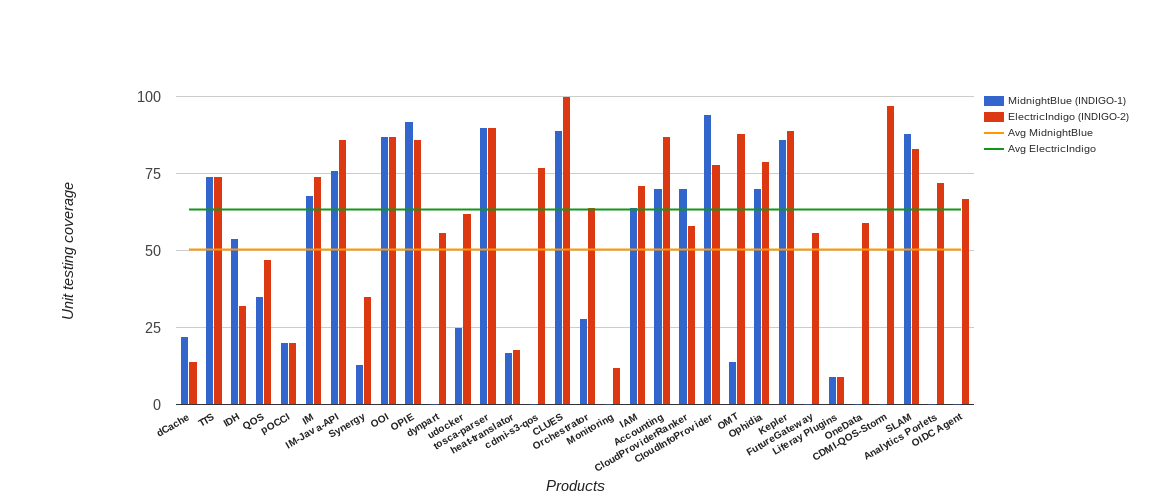
\includegraphics[width=\textwidth]{images/unittest.png}
\caption{Unit testing coverage for the two major INDIGO--DataCloud releases.}
\label{fig:fig_unittest}
\end{figure*}

Fig. \ref{fig:fig_confman} shows the number of products that offer an automated means
for deployment. It shows an increase after the {\sl INDIGO-1} release with specially
in the previous weeks of each of the two major releases.

The evaluation of the software quality is performed by measuring the values of
the metrics and Key Performance Indicators (KPIs) defined based upon the
ISO/IEC 9126 standard. These metrics cover the development, release and
maintenance phases of the software lifecycle. Development and release metrics
are obtained automatically from several sources, such as GitHub and Jenkins CI
service, and graphically displayed as GitHub pages using GrimoireLab framework
\cite{grimoirelab}. Maintenance and user support metrics are collected from the
different sources of data such as GGUS \cite{ggus} and Github Issues.

\begin{figure}
\centering
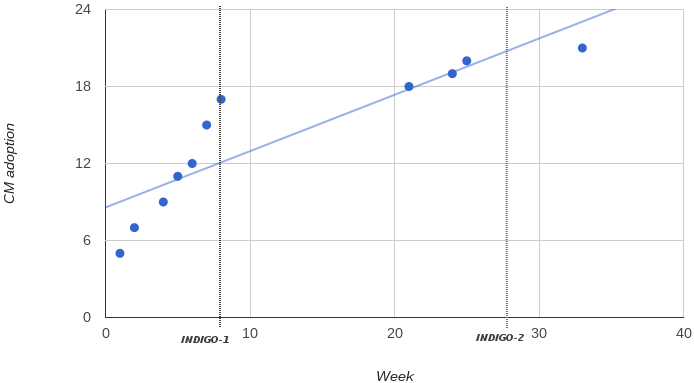
\includegraphics[width=0.45\textwidth, height=50mm]{images/confman.png}
\caption{Trend line showing the adoption of Configuration Management tools throughout the project lifetime.}
\label{fig:fig_confman}
\end{figure}

\subsection{DevOps adoption from user communities}

The experience gathered throughout the project with regard to the adoption of
different DevOps practices is not only useful and suitable for the software related
to the core services in the INDIGO-DataCloud solution, but also applicable to the
development and distribution of the applications coming from the user communities.

Two applications from WP2, DisVis \cite{disvis} and PowerFit \cite{powerfit}, were
integrated into a similar CI/CD pipeline described in section \ref{sec:devops}.
Figure \ref{fig:fig_disvis} shows the pipeline for the Disvis application.

User application developers were provided with both a means to validate the
source code before merging and the creation of a new versioned Docker image,
automatically available in the INDIGO-DataCloud’s application repository.

The novelty introduced in the pipeline above is the validation of the application.
Once the application is deployed as a Docker container, and subsequently uploaded
to the Dockerhub repository, it is instantiated in a new container to be validated.
The application is then executed and the results compared with a set of reference outputs.
Thus this pipeline implementation goes a step forward by testing the application
execution for the last available Docker image in the catalogue.

\begin{figure*}
\centering
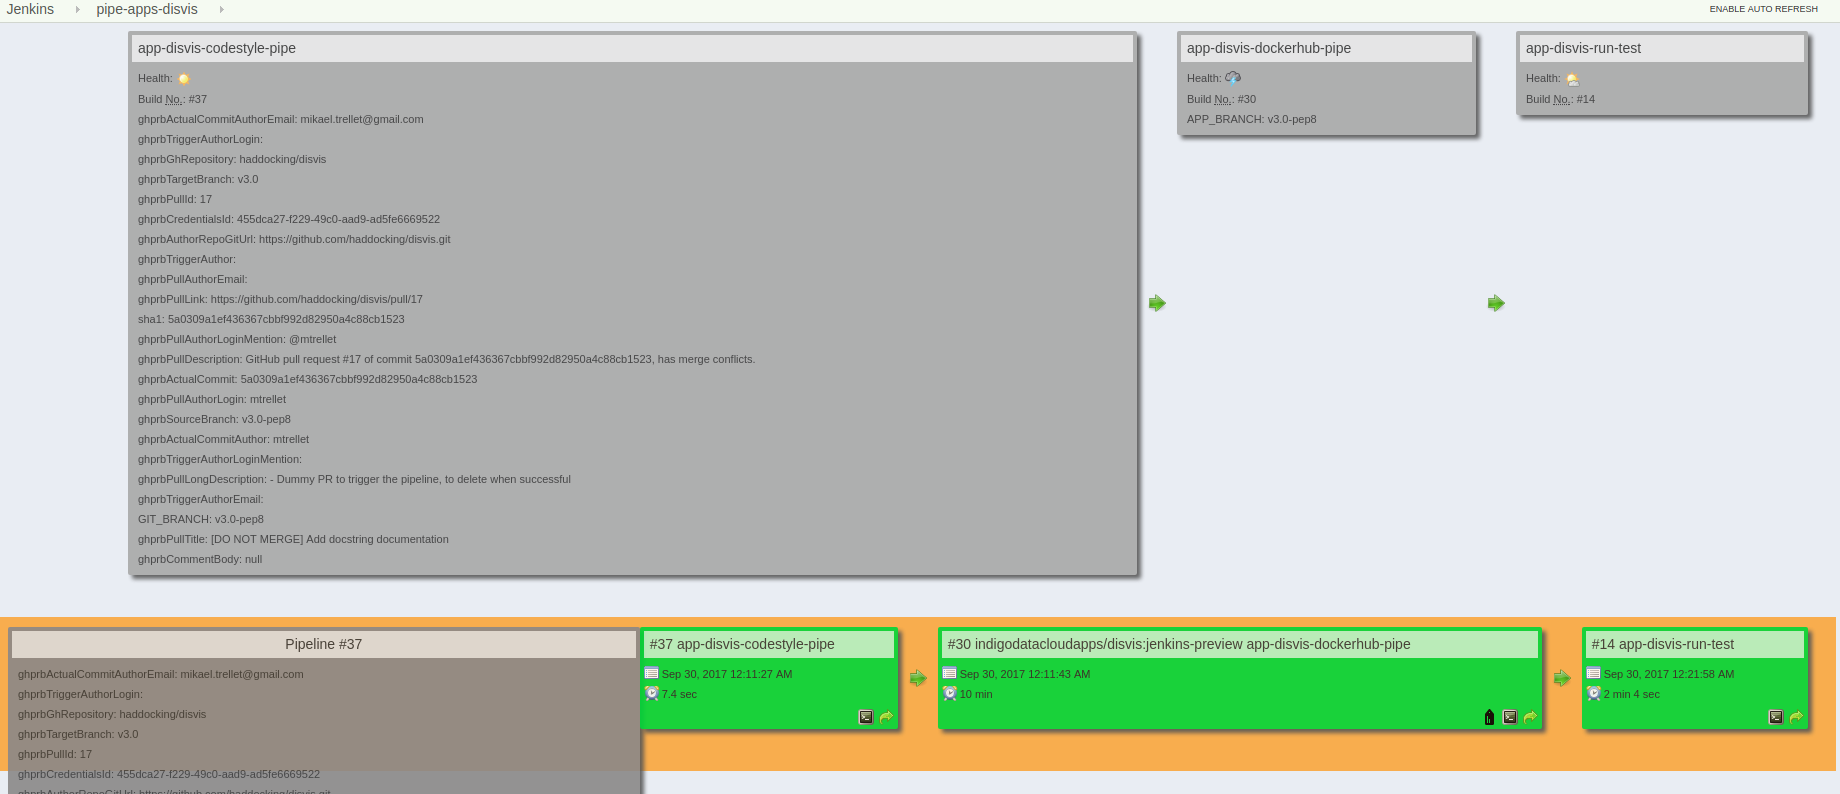
\includegraphics[width=\textwidth]{images/disvis.png}
\caption{DevOps pipeline to distribute Docker images for Disvis application.}
\label{fig:fig_disvis}
\end{figure*}

\subsection{Integration, preview and early adoption}

Two pilot infrastructures are at the disposal of developers and scientific
communities involved in the project. The aim of these testbeds is to test the
level of integration between the components involved in the INDIGO--DataCloud
solution and use cases validation, by deploying and executing the applications
with the last stable version of the software. A map of the Pilot Preview
infrastructure is depicted in Fig. \ref{fig:fig_pilotpreview}, it shows the
resources providers and the components or services they deployed and supported.

\begin{figure*}
\centering
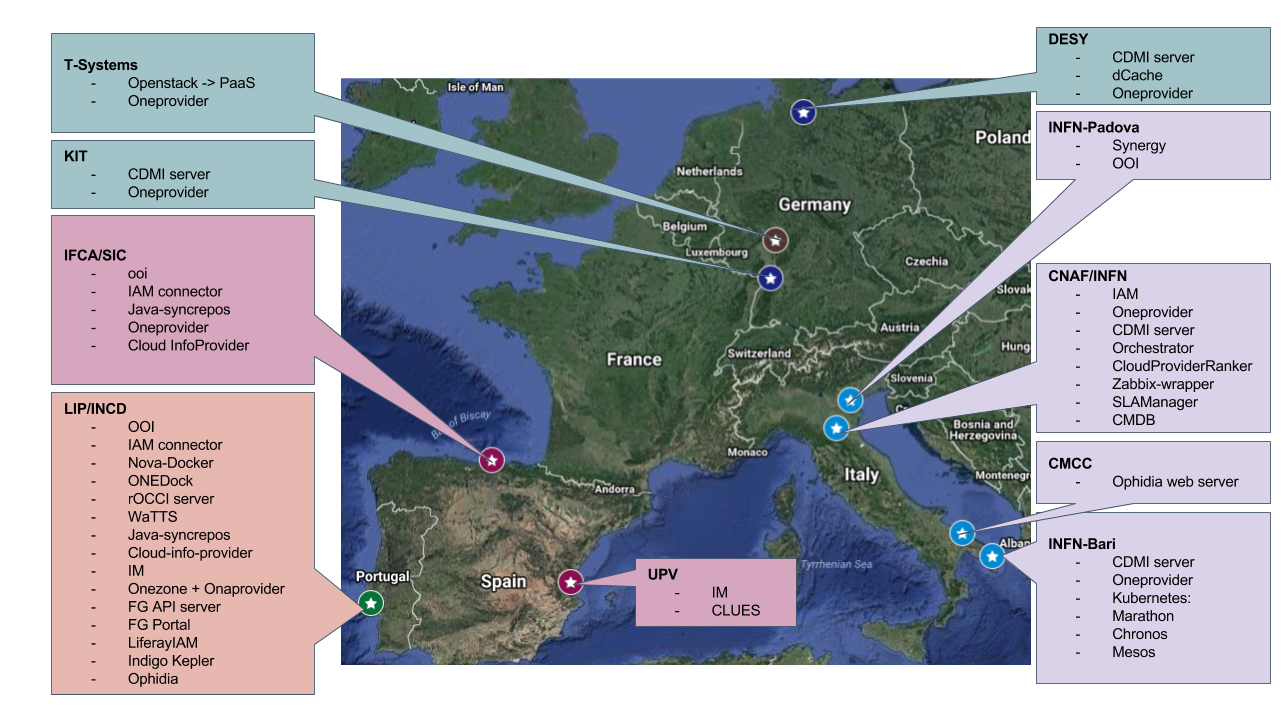
\includegraphics[width=\textwidth]{images/pilotpreview.png}
\caption{Resource centers supporting the Pilot Preview testbed and corresponding
set of deployed INDIGO-DataCloud components or services.}
\label{fig:fig_pilotpreview}
\end{figure*}

The released software is also tested in production environments through the
stage--rollout process. Selected resource providers are requested to install
the most updated stable versions of the software, accessed by their users. The
stage--rollout process is key to detect and mitigate issues that could only
appear in production.

\section{Conclusion}
\label{sec:con}

It is a fact that the European software produced for scientific purposes is
evolving to a more sustainable model where the quality and reliability of
software is being prioritized. Recent software engineering insights, such as
DevOps, are gradually being applied as the open--source collaborative tools
evolve, allowing tighter integrations. The focus of the Software Quality
Assurance procedures has been integrated in the development stage, trying to
detect and correct issues early in the software lifecycle. Automation and
metric analysis are at the base of prompt issue solving. However, post--release
validation, such as integration testbeds and the stage--rollout process, are
also needed to strengthen the software reliability for scientific usage.

\section*{Acknowledgment}

The authors would like to thanks European Commission with the various funded
projects.

\begin{thebibliography}{1}

\bibitem{zhu}
L. Zhu and L. Bass and G. Champlin-Scharff, \emph{DevOps and Its Practices}, 
IEEE Software, vol. 33, no. 3, pp. 32--34, May-June 2016.


\bibitem{cordis:datagrid}
\emph{DataGrid project}, European Community Research and Development
Information Service (CORDIS),
http://cordis.europa.eu/project/rcn/53665\_en.html

\bibitem{globus}
I. Foster and C. Kesselman, \emph{Globus: a Metacomputing Infrastructure
Toolkit}, International Journal of Supercomputer Applications, vol. 11, no. 2,
pp. 115–128, 1997.

\bibitem{datagrid}
L. Momtahan and A. Martin, \emph{e-Science Experiences: Software Engineering
Practice and the EU DataGrid}, in Proc. Asia-Pacific Software Engineering
Conference, Gold Coast, Queensland, Australia, pp. 269-275, IEEE Press,
4-6 Dec. 2002.

\bibitem{agile-manifesto}
\emph{Manifesto for Agile Software Development}, http://agilemanifesto.org

\bibitem{agile}
T. Dingsoyr, \emph{A decade of agile methodologies: Towards explaining agile
software development} in The Journal of Systems and Software, Elsevier Inc,
2012.

\bibitem{cmm}
Paulk et al., \emph{Capability maturity model for software}, Software
Engineering Institute, report CMU/SEI-93-TR-24, ESC-TR-93-177, Feb. 1993.

\bibitem{cordis:egee}
\emph{Enabling Grids for E-sciencE (EGEE)} project, European Community
Research and Development Information Service (CORDIS),
http://cordis.europa.eu/project/rcn/80149\_en.html

\bibitem{cordis:egee2}
\emph{Enabling Grids for E-sciencE-II (EGEE-II)} project, European Community
Research and Development Information Service (CORDIS),
http://cordis.europa.eu/project/rcn/99189\_en.html

\bibitem{cordis:egee3}
\emph{Enabling Grids for E-sciencE-III (EGEE-III)} project, European Community
Research and Development Information Service (CORDIS),
http://cordis.europa.eu/project/rcn/87264\_en.html

\bibitem{glite}
E. Laure et al, \emph{Programming the Grid with gLite}, in Jin, H., Reed, D.A.,
Jiang, W. (eds.) Computational Methods in Science and Technology, vol. 12(1),
pp. 33–45, Scientific Publishers OWN, 2006.

\bibitem{condor}
D. Thain, T. Tannenbaum, M. Livny, \emph{Condor and the grid}, in Grid
Computing: Making the Global Infrastructure a Reality, Chapter 11, pp. 63–70,
Eds. John Wiley \& Sons Inc., 2002.

\bibitem{cordis:etics}
\emph{E-Infrastructure for Testing, Integration and Configuration of Software
(ETICS)} project, European Community Research and Development Information
Service (CORDIS), http://cordis.europa.eu/project/rcn/80138\_en.html

\bibitem{cordis:etics2}
\emph{E-Infrastructure for Testing, Integration and Configuration of Software -
Phase 2 (ETICS 2)} project, European Community Research and Development
Information Service (CORDIS),
http://cordis.europa.eu/project/rcn/86604\_en.html

\bibitem{etics}
A. Di Meglio, M.-E.Bégin, P. Couvares, E. Ronchieri, E. Takacs, \emph{ETICS:
the international software engineering service for the grid}, in Journal of
Physics: Conference Series, Vol. 119, N. 4, IOP Publishing Ltd, 2008.

\bibitem{cordis:emi}
\emph{European Middleware Initiative (EMI)} project, European Community
Research and Development Information Service (CORDIS),
http://cordis.europa.eu/project/rcn/95311\_en.html

\bibitem{iso-9126}
\emph{ISO/IEC 9126 Software Engineering - Product Quality}, International
Organization for Standarization, https://www.iso.org/standard/22749.html

\bibitem{emi-metrics}
\emph{EMI Metrics Specification}, https://goo.gl/CCtY7x


\bibitem{emi-quality-model}
\emph{EMI Quality Model}. Available: https://goo.gl/LdS6fL

\bibitem{cordis:egi-inspire}
\emph{European Grid Initiative: Integrated Sustainable Pan-European
Infrastructure for Researchers in Europe (EGI-InSPIRE)} project, European
Community Research and Development Information Service (CORDIS),
http://cordis.europa.eu/project/rcn/95923\_en.html

\bibitem{egi-qc}
\emph{EGI Quality Criteria}. Available: http://egi-qc.github.io/

\bibitem{mario}
M. David et al, \emph{Validation of Grid Middleware for the European Grid
Infrastructure}, in Journal of Grid Computing, vol. 12, issue 3, pp. 543–558,
Springer, 2014.

\bibitem{cordis:egi-engage}
\emph{Engaging the EGI Community towards an Open Science Commons (EGI-ENGAGE)}
project, European Community Research and Development Information Service
(CORDIS), http://cordis.europa.eu/project/rcn/194937\_en.html

\bibitem{cordis:indigo}
\emph{INtegrating Distributed data Infrastructures for Global ExplOitation
(INDIGO-DataCloud)} project, European Community Research and Development
Information Service (CORDIS),
http://cordis.europa.eu/project/rcn/194882\_en.html

\bibitem{indigo-dockerhub}
\emph{INDIGO-DataCloud DockerHub repository},
https://hub.docker.com/u/indigodatacloud

\bibitem{indigo-d31}
\emph{Initial Plan for WP3} INDIGO-DataCloud Deliverable 3.1,
https://www.indigo-datacloud.eu/documents/initial-plan-wp3-d31

\bibitem{indigo-jenkins}
\emph{INDIGO-DataCloud Jenkins CI service},
https://jenkins.indigo-datacloud.eu:8080/

\bibitem{indigo-github}
\emph{INDIGO-DataCloud GitHub Source Code repository},
https://www.github.com/indigo-dc

\bibitem{indigo-gitbook}
\emph{INDIGO-DataCloud GitBook Documentation repository},
https://www.gitbook.com/@indigo-dc

\bibitem{indigo-puppet}
\emph{INDIGO-DataCloud PuppetForge repository},
https://forge.puppet.com/indigodc

\bibitem{indigo-ansible}
\emph{INDIGO-DataCloud Ansible Galaxy repository},
https://galaxy.ansible.com/indigo-dc/

\bibitem{grimoirelab}
\emph{GrimoireLab}, http://grimoirelab.github.io/

\bibitem{ggus}
\emph{Global Grid User Support (GGUS)}, https://www.ggus.eu/

\bibitem{disvis} G.C.P. Van Zundert, A.M.J.J. Bonvin,
DisVis: quantifying and visualizing the accessible interaction space of distance
restrained biomolecular complexes, Bioinformatics 31 (2015) 3222–3224

\bibitem{powerfit} G.C.P. Van Zundert, A.M.J.J. Bonvin,
Fast and sensitive rigid-body fitting into cryo-EM density maps with PowerFit,
AIMS Biophys. 2 (2015) 73–87.

\end{thebibliography}

\begin{IEEEbiography} [{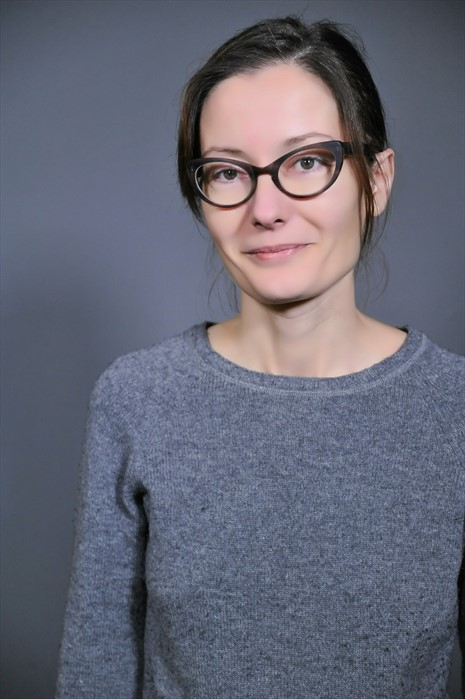
\includegraphics[width=1in,height=1.25in,clip,keepaspectratio]{images/Ronchieri}}]{Elisabetta Ronchieri}
is a Computer Science Engineer at INFN (Istituto Nazionale di Fisica Nucleare - National Institute of Nuclear Physics) CNAF. She holds a PhD in Automation, Robotics and Bioengineering from the University of Pisa. Her main area of interest include software engineering issues, such as software quality and software prediction model. She is also interested in (big and open) data analysis by using techniques coming from various theories, such as Machine Learning.
\end{IEEEbiography}

% if you will not have a photo at all:
\begin{IEEEbiography}{Pablo Orviz Fernandez}
Biography text here.
\end{IEEEbiography}

\begin{IEEEbiography}[{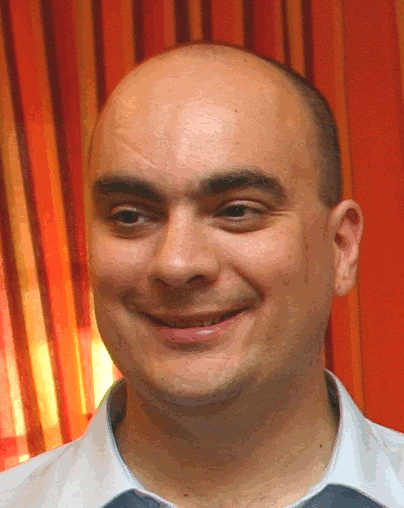
\includegraphics[width=1in,height=1.25in,clip,keepaspectratio]{images/mario-david}}]{Mario David}
Mario David is a research associate at LIP. He holds a PhD in Experimental Particle Physics from the University of Lisbon.
Member of DEEP-HybridDatacloud project as Work Package leader of Testbed and integration with EOSC services. Member of EOSC-Hub project and
of the Portuguese National Computing Distributed Infrastructure.
He held a research associate position at Institut de Physique du Globe de Paris (IPGP/CNRS) as Scientific Software Developer for the VERCE project, in particular in the data intensive use cases for seismology.
He was been actively involved in the Validation, Quality Assurance and testing of middleware, in regional and global operations.
\end{IEEEbiography}

\begin{IEEEbiography}{Doina Cristina Duma}
Biography text here.
\end{IEEEbiography}


\begin{IEEEbiography}[{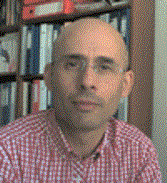
\includegraphics[width=1in,height=1.25in,clip,keepaspectratio]{images/jorge-gomes}}]{Jorge Gomes}
Jorge Gomes is a computing researcher at LIP. He worked in the development of advanced data acquisition systems at CERN, and participated in pioneering projects in the domain of digital satellite data communications, IP over ATM, and advanced videoconferencing over IP networks. Since 2001 he has participated in numerous projects regarding distributed computing, networks and security in Europe and Latin America. He is the head of the LIP Advanced Computing and Digital Infrastructures Group and technical coordinator of the Portuguese National Grid Infrastructure, representative of Portugal in the Council of the European Grid Infrastructure (EGI) and responsible for the Portuguese participation in IBERGRID, that joins Portuguese and Spanish distributed computing infrastructures.
\end{IEEEbiography}

\begin{IEEEbiography}[{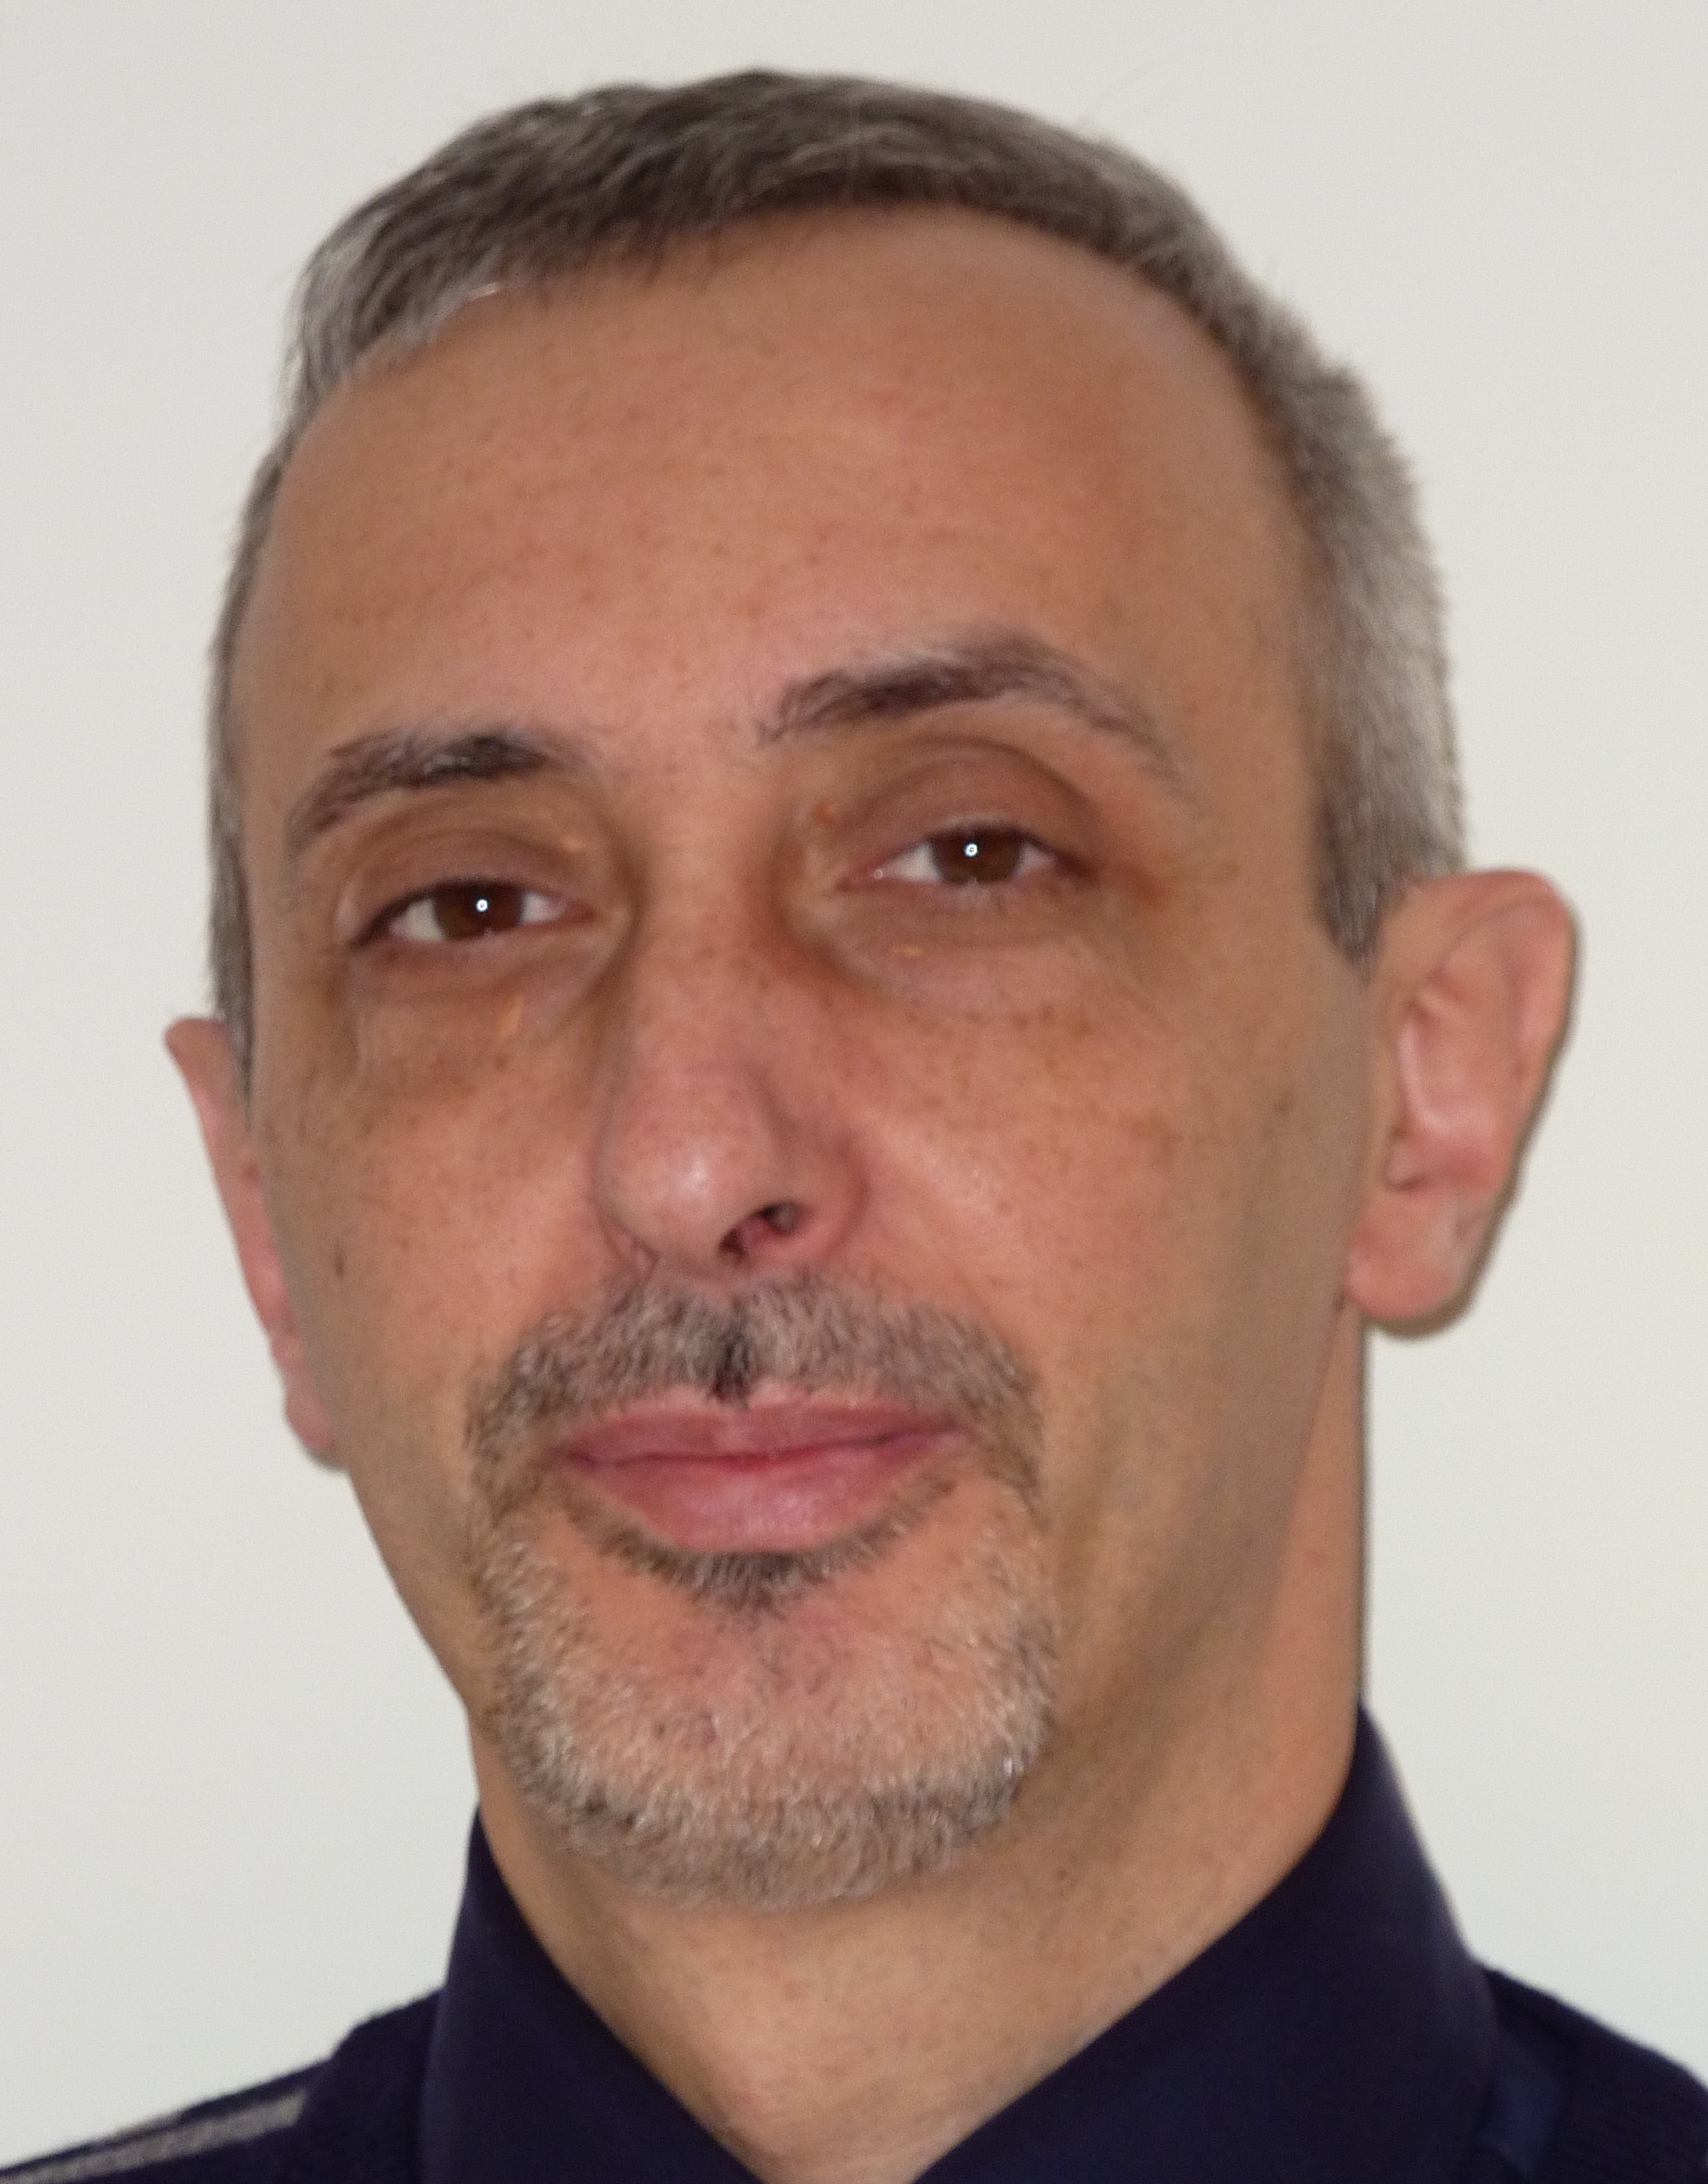
\includegraphics[width=1in,height=1.25in,clip,keepaspectratio]{images/DavideSalomoni}}]{Davide Salomoni}
Davide SAlomoni is Director of Technology at the Italian National Institute for Nuclear Physics (INFN). He has 27 years of international experience in private and public environments related to distributed computing and communication technologies. He currently leads the Software Development and Distributed Systems department at CNAF, the INFN National Center Dedicated to research and development on IT technologies, located in Bologna, Italy. He was Project Coordinator of INDIGO-DataCloud, a project funded by the EC Horizon2020, that developed innovative open source computing and storage solutions.
\end{IEEEbiography}





\end{document}


